% !TEX root =../thesis-letomes.tex

\chapter{Discussion}

\section{Errors Found in Old BSc Code}
We found some mathematical errors in the old code; argue for why they don’t invalidate the old results

\section{Stability of Trajectories: Lyapunov Exponent}
argue for correctness of method and trustworthiness of trajectories by quantifying the inherent chaos: Basically, we are addressing the fact that this is a numerical simulation, and therefore a compressed view of the real thing. It is important to argue that that compression is not too much.

\subsection{Sensitivity analysis}

In our experiments, we found that our paths were diverging pretty heavily given relatively small changes to initial conditions. This was a concern in the original project as well, but was not fully explored then. It is important to quantify the chaotic nature of a system like this, since we are dealing with numerical simulation, which will always have some error associated with it. One takes steps to minimize such errors, often sacrificing computing performance to do so. However, if a system has an error of magnitude say \(\num{1e-8}\), and the system is so chaotic that errors of or \(\num{1e-9}\) at one point early in the trajectory effect meaningful changes further down the line, then the path is near invalid! Therefore, it is important to try to quantify the chaos of a system (in this case our simulator), to provide assurances that the resulting paths have any meaningful truth to them. We have done this by calculating Lyapunov exponents for the system, explained below.

\subsection{Lyapunov Exponent}

The Lyapunov exponent describes the rate of change as time goes on between time series with infinitesimally different starting conditions, as they progress. The method is to compute a set of trajectories, and take the difference between them at set points in time (euclidean distance when dealing with higher dimensions). In a chaotic system, these two trajectories should diverge from each other at some exponential rate, and the Lyapunov exponent is that rate. If we want to trust our results, we want that number to be as low as possible. 

\subsection{Implementation}

We ran several simulations of known good trajectories, with their starting conditions very slightly perturbed, in such a way that the trajectories initially diverged from each other by a value less that 1e-8, chosen as the square root of the precision of the 64-bit floating point numbers that describe the coordinates. The trajectories were then discretized to synchronize the variable length of the time steps, and then compared in pairs, tick by tick, yielding a list of euclidean distances at each step. We then took the natural logarithm of these lists, giving us the plots pictured in figure \ref{fig:long_leto_slope} and \ref{fig:hohmann_slope}. The graph varied heavily depending on the gist of the trajectory in question, with trajectories that made multiple passes near earth giving the tooth-like distance graphs pictured in fig. \ref{fig:long_leto_slope}. Trajectories that did not visit earth more than once gave much more `normal' results, given what we see in the literature pertaining to Lyapunov exponent analysis. Clearly, passing into the LEO domain has a powerful stabilizing effect on the the chaotic system, acting like a focal lens for the trajectories passing through. It's not completely trivial to give a Lyapunov exponent from this, but since the individual tooth-segments have a more or less equivalent slope, we simply took the average slope of the first five teeth. A deeper look into this cyclical chaos would be interesting, but we did not delve deeper than this.

A good heuristic for whether or not our paths are precise enough would be a measure that would give some confidence interval for final position, given the gist of a trajectory, and the duration of flight along it. We have calculated such measures, presented in fig. \todoref{reflyapunov heuristic}.

\begin{figure}
    \centering
    \subfloat[a straight-forward Hohmann transfer]{
        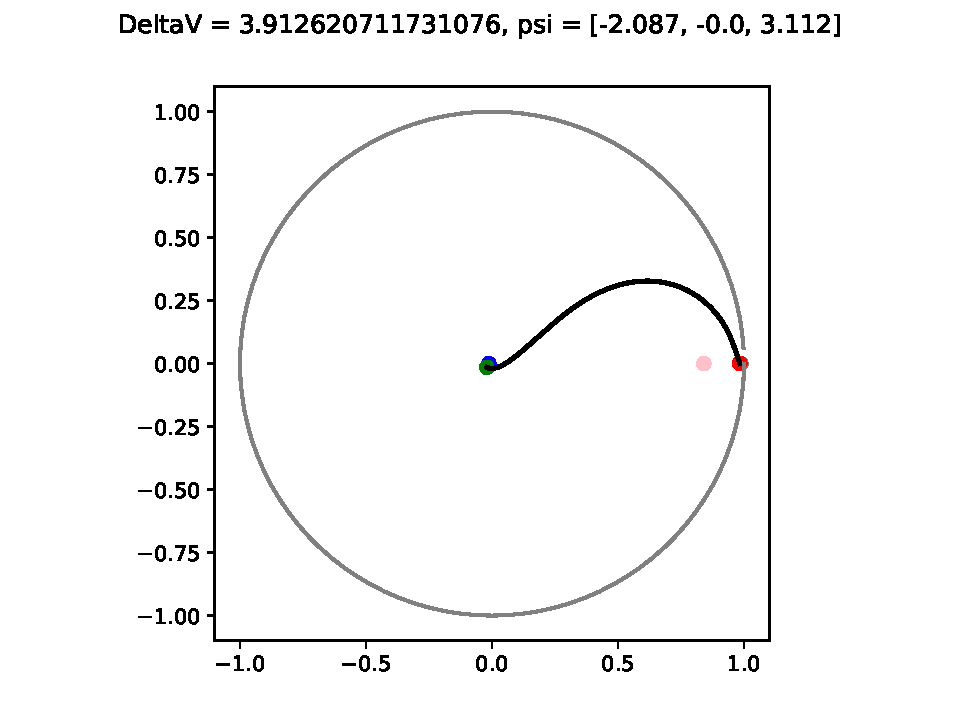
\includegraphics[width=0.46\linewidth]{fig/path_hohmann_non-inertial}
        \label{fig:path_hohmann_non-inertial}
    }
    \hfill
    \subfloat[the rate of separation between infinitesimally perturbed versions of the Hohmann transfer]{
        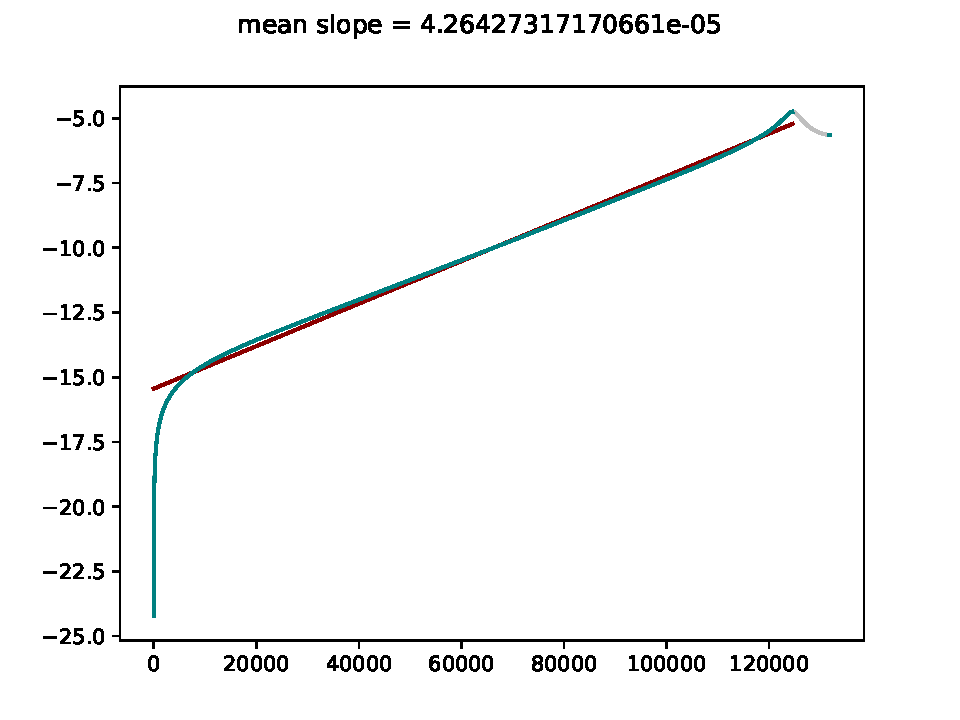
\includegraphics[width=0.46\linewidth]{fig/hohmann_slope}
        \label{fig:hohmann_slope}
    }
    \\
    \subfloat[a relatively long LETO path]{
        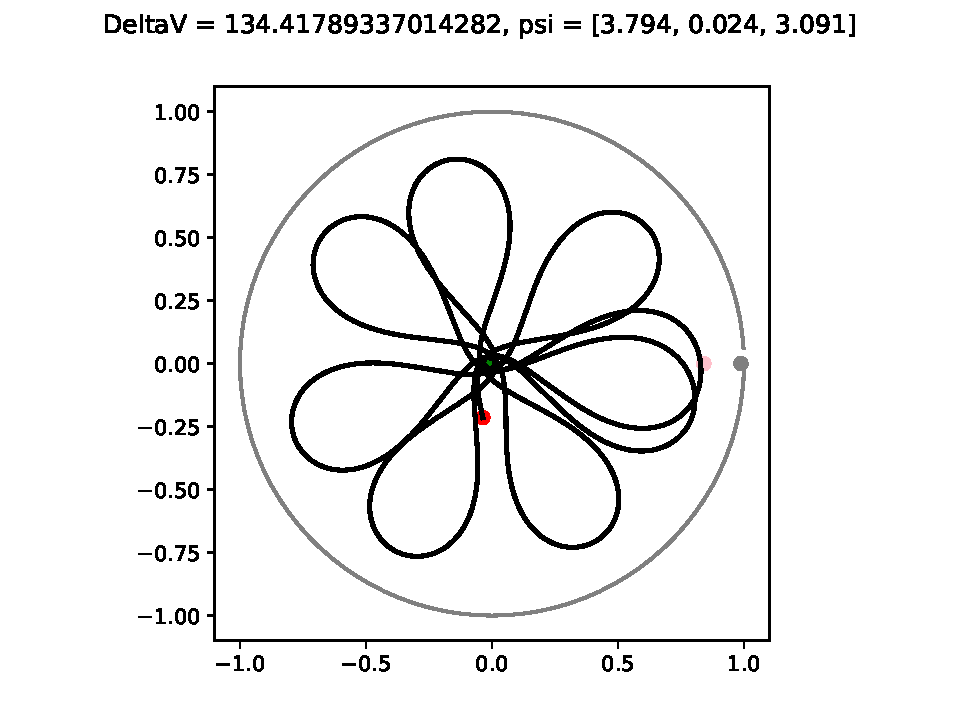
\includegraphics[width=0.46\linewidth]{fig/path_long_leto_non-inertial}
        \label{fig:path_long_leto_non-inertial}
    }
    \hfill
    \subfloat[the rate of separation of two infinitesimally perturbed versions of the long LETO]{
        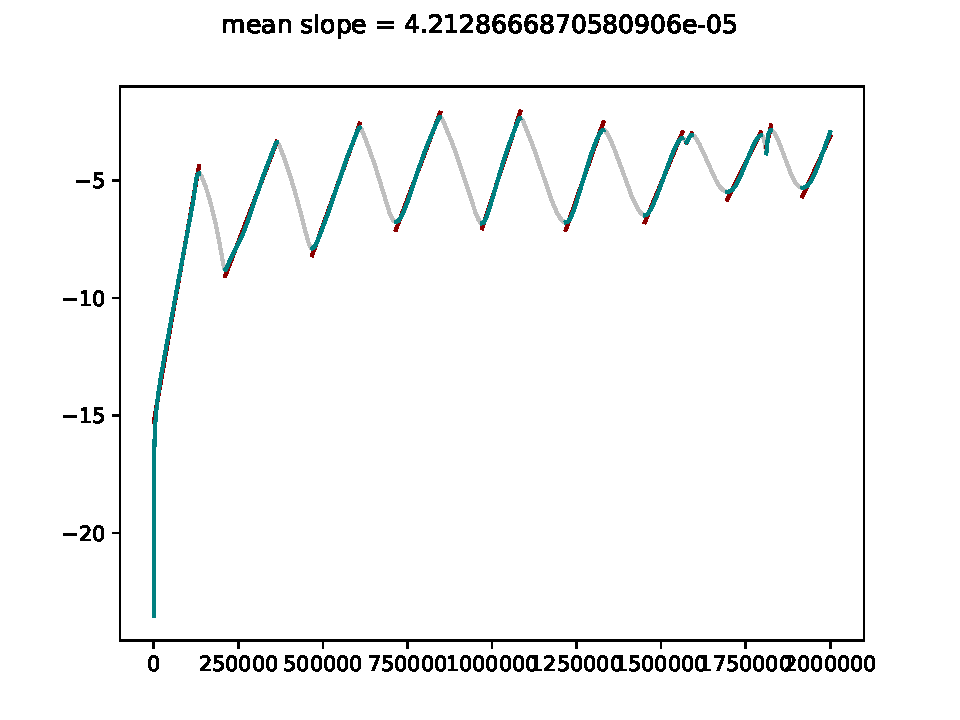
\includegraphics[width=0.46\linewidth]{fig/long_leto_slope}
        \label{fig:long_leto_slope}
    }
    \caption{Examples of some of the different types of transfers that are possible within the model. Each of these were taken as starting points, and simulated again with slightly perturbed starting conditions. The difference between these perturbations were then measured, and plotted in \textbf{b} and \textbf{d}, on a logarithmic scale. The slope of these plots is the lyapunov exponent. We can see that passing into a deep gravity well has a stabilizing effect on the chaos in the system.}
    \label{fig:lyapunov}
\end{figure} 

% \begin{figure}
%     \centering
%     \subfloat[test-a]{
%         
\includegraphics[width=0.46\linewidth]{temp/img1}
%         \label{img1}
%     }
%     \hfill
%     \subfloat[test-b]{
%         
\includegraphics[width=0.46\linewidth]{temp/img2}
%         \label{img2)}
%     }
%     \\
%     \subfloat[test-c]{
%         
\includegraphics[width=0.46\linewidth]{temp/img3}
%         \label{img3}
%     }
%     \hfill
%     \subfloat[test-d]{
%         
\includegraphics[width=0.46\linewidth]{temp/img4}
%         \label{img4)}
%     }
%     \caption{Overall caption}
%     \label{fig:somelabel}
% \end{figure} 

% \begin{figure}
%     \centering
%     \subfloat[Figure a) caption]{
%         
\includegraphics[width=0.46\linewidth]{temp/img1}
%         \label{fig:Image a) filename}
%     }
%     \hfill
%     \subfloat[Figure b) caption]{
%         
\includegraphics[width=0.46\linewidth]{temp/img2}
%         \label{Image b) filename)}
%     }
% \end{figure} 
%     \\
%     \centering
%     \subfloat[Figure c) caption]{
%         
\includegraphics[width=0.46\linewidth]{temp/img3}
%         \label{fig:Image c) filename}
%     }
%     \hfill
%     \subfloat[Figure d) caption]{
%         
\includegraphics[width=0.46\linewidth]{temp/img4}
%         \label{Image d) filename)}
%     }
%     \caption{field 1:default=Overall caption}
%     \label{fig:Overall figure label}
% \end{figure}


\section{Brute Force vs. ES}
In this section, we will examine the usefulness of using the ES algorithm over the brute force alternative. Do we get anything out of estimating a gradient? Do our results’ quality scale with a more complex model?

The ES method is in the general case a more intelligent of searching for these things. However, its not a magical panacea that just spits out fabulous results from a naive application. The brute force method took advantage of a lot of human intuition in terms of where to search. We gave it a limited fan of possibilities in a region that we knew to be reasonable. The ES algorithm definitely gave the best results when we imposed equivalent limitations on it.

\section{Delta-v Travel Time Trade-off}
Delta-v Travel Time Trade-off. Plot this, if we can get enough different successful trajectories. What does that plot look like?

\section{Performance Optimization}
was PaGMO a good choice? Is it a reasonable problem to run on GPU or are we transporting too much data?

\section{Self-evaluation}
Was our time well spent? Did we gain anything from our "reinventing the wheel", re-implementing the lunar simulator? Should we have focused on running on the old code without delving into it?